% figS_pipeline_schematic.tex
% ---------------------------------------------------------------------------
% Supplementary schematic of the unified UKB whole-genome SPHERE pipeline.
% Draft. Renders to revision/figures/figS_pipeline_schematic_draft.pdf
%
% Design intent: the single point a reader must take away is that after the
% rotation the real and synthetic lanes NEVER exchange information again --
% the synthetic principal components are estimated from the synthetic matrix
% alone. The two lanes are therefore drawn as parallel columns that only meet
% at the three dashed comparison bars (CLAIM 1/2/3). The rotation itself sits
% INSIDE the synthetic lane, since it is what creates that lane; the real lane
% carries the filtered matrix through unchanged.
%
% Colors match figure3_ukb_v2.py: REAL #2166AC, SPHERE #D73027, ColShuffle
% #1A9850, grey #999999. Blue/red/green on white is safe for deuteranopia and
% protanopia at these luminances; the two lanes are additionally distinguished
% by position and by solid vs dashed borders, so color is never load-bearing.
% ---------------------------------------------------------------------------
\documentclass[border=6pt]{standalone}
\usepackage{tikz}
\usepackage{amsmath}
\usepackage{helvet}
\renewcommand{\familydefault}{\sfdefault}
\usepackage[T1]{fontenc}
\usetikzlibrary{arrows.meta,positioning,fit,backgrounds,calc}

\definecolor{realc}{HTML}{2166AC}
\definecolor{synthc}{HTML}{D73027}
\definecolor{greyc}{HTML}{999999}
\definecolor{realbg}{HTML}{E8EFF7}
\definecolor{synthbg}{HTML}{FBEAE8}
\definecolor{sharebg}{HTML}{F2F2F2}

\begin{document}
% The CLAIM labels are set in a 19mm column, narrow enough that TeX starts
% hyphenating ("ro-tated"). Hyphenation is off for the whole figure instead.
\hyphenpenalty=10000
\exhyphenpenalty=10000
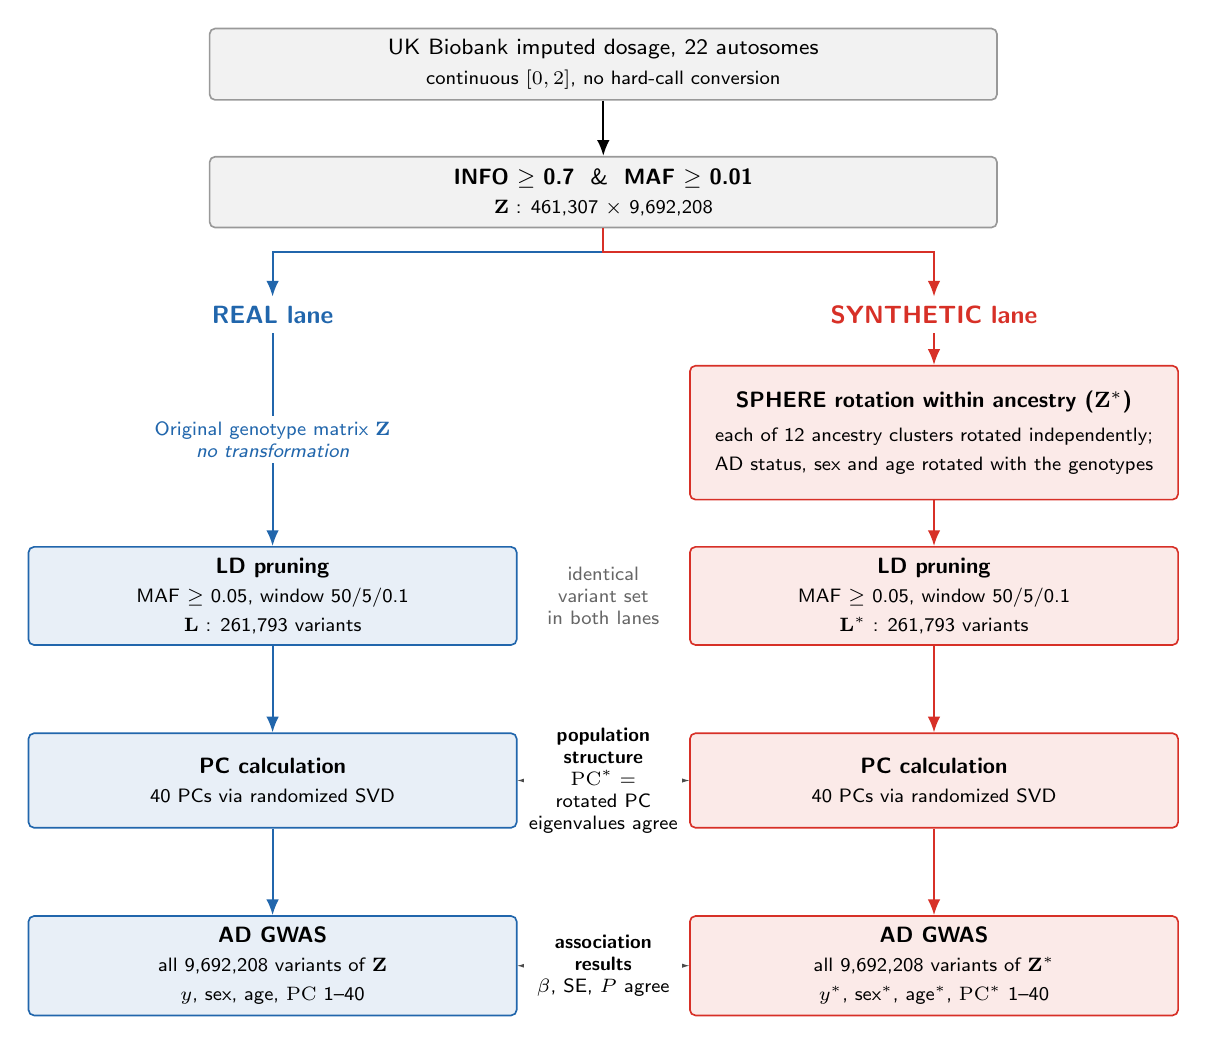
\begin{tikzpicture}[
  font=\footnotesize,
  node distance=0pt,
  box/.style={draw,rounded corners=2pt,align=center,inner sep=4pt,
              minimum width=62mm,minimum height=12mm,line width=0.6pt},
  realbox/.style={box,draw=realc,fill=realbg},
  synthbox/.style={box,draw=synthc,fill=synthbg},
  sharebox/.style={box,draw=greyc,fill=sharebg,minimum width=100mm,
                   minimum height=9mm},
  arr/.style={-{Latex[length=2mm,width=1.6mm]},line width=0.7pt},
  realarr/.style={arr,draw=realc},
  syntharr/.style={arr,draw=synthc},
  claim/.style={latex-latex,dashed,line width=0.7pt,draw=black!70},
  % text width is capped so the label stays inside the 22mm centre channel and
  % never covers a lane box border.
  claimlab/.style={fill=white,inner sep=1.5pt,align=center,text width=19mm,
                   font=\scriptsize\bfseries},
]

% ---------- geometry -------------------------------------------------------
% Lane centres. A 62mm lane box centred at +-42mm leaves a 22mm channel in the
% middle for the CLAIM labels. The shared boxes are deliberately narrower than
% the lane span (100mm) so the head of the diagram does not read as one long bar.
\def\lx{-42mm}   % real lane centre
\def\rx{42mm}    % synthetic lane centre

% ---------- shared input ---------------------------------------------------
\node[sharebox] (raw) at (0,0)
  {UK Biobank imputed dosage, 22 autosomes\\[1pt]
   \scriptsize continuous $[0,2]$, no hard-call conversion};

\node[sharebox,below=7mm of raw] (filt)
  {\textbf{INFO $\geq$ 0.7} \ \& \ \textbf{MAF $\geq$ 0.01}\\[1pt]
   \scriptsize $\mathbf{Z}$ : 461{,}307 $\times$ 9{,}692{,}208};
\draw[arr] (raw) -- (filt);

% ---------- lane headers ---------------------------------------------------
\node[font=\small\bfseries,text=realc] (rhead)
      at ($(filt.south)+(\lx,-11mm)$) {REAL lane};
\node[font=\small\bfseries,text=synthc] (shead)
      at ($(filt.south)+(\rx,-11mm)$) {SYNTHETIC lane};
\draw[realarr] (filt.south) -- ++(0,-3mm) -| (rhead.north);
\draw[syntharr] (filt.south) -- ++(0,-3mm) -| (shead.north);

% ---------- rotation: the first step OF the synthetic lane -----------------
% The rotation is what creates the synthetic lane, so it belongs inside it
% rather than upstream of the split. The real lane carries Z through unchanged.
% What the reader needs from this box is not the algebra (that lives in Methods)
% but three operational facts: how the 12 clusters were defined, that each one is
% rotated by its own key so no individual is mixed across ancestry, and that the
% phenotype and the non-PC covariates travel through the same rotation.
% Ward's method, the 40k subsample used to build the tree and the 1,000-member
% minimum cluster size are all left to the caption; the box carries only the
% three facts a reader needs to follow the diagram.
% The output symbol rides in the title, mirroring "Original genotype matrix Z"
% on the real side, so the two lanes are named by their matrix at a glance.
\node[synthbox,below=4mm of shead,minimum height=17mm] (rot)
  {\textbf{SPHERE rotation within ancestry ($\mathbf{Z}^{*}$)}\\[3pt]
   \scriptsize each of 12 ancestry clusters rotated independently;\\[1pt]
   \scriptsize AD status, sex and age rotated with the genotypes};
\draw[syntharr] (shead) -- (rot);

% ---------- independent pruning + PCA --------------------------------------
% 4mm gap + 17mm rotation box + 6mm gap = 27mm, so the pruning row lines up in
% both lanes even though the real lane has nothing in the rotation row.
\node[realbox,below=27mm of rhead] (rprune)
  {\textbf{LD pruning}\\[1pt]
   \scriptsize MAF $\geq$ 0.05, window 50/5/0.1\\[1pt]
   \scriptsize $\mathbf{L}$ : 261{,}793 variants};
\node[synthbox] (sprune) at (rprune -| shead)
  {\textbf{LD pruning}\\[1pt]
   \scriptsize MAF $\geq$ 0.05, window 50/5/0.1\\[1pt]
   \scriptsize $\mathbf{L}^{*}$ : 261{,}793 variants};
% Stated as what the real lane IS rather than as what was not done to it: the
% earlier "carried through unrotated" invited the reader to ask why the rotation
% was skipped here, or whether Z travelled through the rotation at all.
\draw[realarr] (rhead) -- (rprune)
  node[midway,fill=white,inner sep=2pt,align=center,font=\scriptsize,
       text=realc] {Original genotype matrix $\mathbf{Z}$\\\itshape
                    no transformation};
\draw[syntharr] (rot) -- (sprune);

\node[realbox,below=11mm of rprune] (rpca)
  {\textbf{PC calculation}\\[1pt]
   \scriptsize 40 PCs via randomized SVD};
\node[synthbox] (spca) at (rpca -| shead)
  {\textbf{PC calculation}\\[1pt]
   \scriptsize 40 PCs via randomized SVD};
\draw[realarr] (rprune) -- (rpca);
\draw[syntharr] (sprune) -- (spca);

% ---------- GWAS -----------------------------------------------------------
\node[realbox,below=11mm of rpca] (rgwas)
  {\textbf{AD GWAS}\\[1pt]
   \scriptsize all 9{,}692{,}208 variants of $\mathbf{Z}$\\[1pt]
   \scriptsize $y$, sex, age, $\mathrm{PC}$ 1--40};
\node[synthbox] (sgwas) at (rgwas -| shead)
  {\textbf{AD GWAS}\\[1pt]
   \scriptsize all 9{,}692{,}208 variants of $\mathbf{Z}^{*}$\\[1pt]
   \scriptsize $y^{*}$, sex$^{*}$, age$^{*}$, $\mathrm{PC}^{*}$ 1--40};
\draw[realarr] (rpca) -- (rgwas);
\draw[syntharr] (spca) -- (sgwas);

% The GWAS runs on the full filtered matrix, not on the pruned subset; the
% pruned subset only supplies the PCs. Stated in the box labels rather than
% drawn, because a second set of long routed arrows made the lane structure
% harder to read, which is the one thing this figure exists to convey.

% ---------- claim connectors ----------------------------------------------
% The pruned sets are now identical (261,793 variants) after float64 LD-pruning
% resolved the two float32 threshold ties. The centre label states this.
\node[claimlab,draw=none,fill=none,text=black!60] at
  ($(rprune.east)!0.5!(sprune.west)$)
  {\mdseries identical\\variant set\\\mdseries in both lanes};
% Two comparisons, in the order they are claimed: population structure is
% preserved, and the association scan built on it reproduces. Named rather than
% numbered, because with the pruning bar gone a "CLAIM 2 / CLAIM 3" pair would
% start at 2, and the CLAIM 1-3 numbering in docs/PIPELINE_UNIFIED_Q_PROPOSAL.md
% refers to pipeline steps, not to the bars drawn here.
\draw[claim] (rpca.east) -- node[claimlab] {population structure\\
  \scriptsize\mdseries $\mathrm{PC}^{*}$ = rotated PC\\\scriptsize\mdseries
  eigenvalues agree} (spca.west);
% Hit count (646/646/646) is in the caption, not on the bar.
\draw[claim] (rgwas.east) -- node[claimlab] {association results\\
  \scriptsize\mdseries $\beta$, SE, $P$ agree} (sgwas.west);

% The explanatory footer that used to sit here was removed: the point it made
% (lanes independent after the rotation, dashed bars are comparisons) is already
% carried by the layout itself and belongs in the figure caption, not the panel.

\end{tikzpicture}
\end{document}
